\documentclass[11pt,a4paper]{article}

\usepackage[utf8]{inputenc}
\usepackage[spanish,es-tabla]{babel}
\usepackage{amsmath,amssymb,amsfonts}
\usepackage{booktabs}
\usepackage{graphicx}
\usepackage{geometry}
\usepackage{xcolor}
\usepackage{hyperref}
\usepackage{listings}
\usepackage{caption}
\usepackage{subcaption}
\usepackage{microtype}
\usepackage{float}

\geometry{top=2.5cm, bottom=2.5cm, left=2.5cm, right=2.5cm}

\hypersetup{
    colorlinks=true,
    linkcolor=blue!70!black,
    citecolor=red!70!black,
    urlcolor=blue!60!black
}

\title{\textbf{Comparación Experimental de Colas de Prioridad: Fibonacci Heaps, Hollow Heaps, Pairing Heaps y Rank-Pairing Heaps}\\[0.3cm]
\large Análisis de Rendimiento, Comportamiento de Caché y Patrones de Acceso a Memoria}

\author{
    \textbf{Matias Sanchez} \and \textbf{Andre Contreras}\\[0.2cm]
    \textit{Universidad de Ingeniería y Tecnología (UTEC)}\\
    \textit{Ciencia de la Computación --- Proyecto Final de EDA}\\[0.25cm]
    \small Repositorio GitHub: \url{https://github.com/andre749/ProyectoFinalEda}
}
\date{Noviembre de 2026}

\begin{document}

\maketitle

\begin{abstract}
Las colas de prioridad con soporte eficiente para la operación \texttt{decrease-key} son componentes esenciales en algoritmos clásicos de grafos como Dijkstra y Prim. Aunque el montículo de Fibonacci (\textit{Fibonacci Heap}) garantiza asintóticamente $O(1)$ amortizado para \texttt{decrease-key} y $O(\log n)$ para \texttt{extract-min}, su alta complejidad estructural suele resultar ineficiente en implementaciones prácticas. En este trabajo evaluamos experimentalmente cuatro estructuras de datos: \textit{Fibonacci Heap}, \textit{Hollow Heap} (variante \textit{multi-root 1-parent}), \textit{Pairing Heap} y \textit{Rank-Pairing Heap} (Tipo 2). Todas las estructuras fueron implementadas bajo una interfaz unificada y testeadas sobre diversas topologías de grafos (dispersos, densos y mallas 2D) con hasta $50\,000$ vértices y más de $500\,000$ aristas. Adicionalmente, se presenta un análisis en profundidad de la huella de memoria, la localidad espacial/temporal y el impacto del comportamiento de la jerarquía de caché (L1/L2) en hardware moderno. Los resultados confirman que el \textit{Pairing Heap} es consistentemente la estructura más rápida en tiempo real de reloj (superando a Fibonacci por factores de entre $3\times$ y $5\times$), mientras que el \textit{Rank-Pairing Heap} emerge como la alternativa más competitiva cuando se requiere balancear garantías asintóticas estrictas con baja sobrecarga de punteros.
\end{abstract}

\vspace{0.5cm}
\tableofcontents
\newpage

% ==============================================================================
\section{Introducción y Marco Teórico}
% ==============================================================================

El estudio de colas de prioridad avanzadas surge históricamente de la necesidad de optimizar algoritmos voraces de caminos mínimos y árboles de expansión mínima. La introducción del \textit{Fibonacci Heap} por Fredman y Tarjan \cite{fredman1987fibonacci} demostró teóricamente que el algoritmo de Dijkstra puede ejecutarse en tiempo $O(E + V \log V)$, reduciendo la cota previa de $O(E \log V)$.

No obstante, como demostraron Larkin, Sen y Tarjan \cite{larkin2014back}, las garantías asintóticas en el modelo RAM de costo uniforme ocultan factores constantes significativos y pasan por alto el coste de transferencias en la jerarquía de memoria. En las arquitecturas multinúcleo contemporáneas, el costo de un fallo de caché hacia memoria principal (DRAM) puede superar los 150--200 ciclos de CPU, penalizando severamente estructuras con patrones dispersos de persecución de punteros (\textit{pointer chasing}).

Con el fin de mitigar la complejidad del \textit{Fibonacci Heap}, se han propuesto alternativas fundamentales:
\begin{enumerate}
    \item \textbf{Pairing Heap \cite{fredman1986pairing}:} Estructura autoconforme de árbol binario de diseño excepcionalmente simple, cuya cota amortizada exacta para \texttt{decrease-key} se ubica entre $o(\log n)$ y $O(\log \log n)$ o $O(2^{2\sqrt{\log \log n}})$ \cite{pettie2005towards}, pero cuyo rendimiento en benchmarks suele ser el estándar a batir.
    \item \textbf{Rank-Pairing Heap \cite{haeupler2011rank}:} Diseñado por Haeupler, Sen y Tarjan para combinar la simplicidad de punteros de los \textit{Pairing Heaps} con las garantías formales de los \textit{Fibonacci Heaps}, empleando rangos enteros y representaciones en \textit{half-trees}.
    \item \textbf{Hollow Heap \cite{hansen2017hollow}:} Propuesto por Hansen, Kaplan, Tarjan y Zwick, sustituye las cascadas de cortes por un enfoque de eliminación perezosa (\textit{lazy deletion}) donde los nodos modificados se convierten en nodos huecos (\textit{hollow}), logrando un diseño desacoplado en grafos dirigidos acíclicos (DAGs) o colecciones de árboles.
\end{enumerate}

\begin{table}[h!]
\centering
\small
\caption{Complejidades asintóticas teóricas (peor caso / amortizado).}
\label{tab:teoria}
\begin{tabular}{lccccc}
\toprule
\textbf{Estructura} & \textbf{Insert} & \textbf{Find-Min} & \textbf{Extract-Min} & \textbf{Decrease-Key} & \textbf{Meld} \\
\midrule
Fibonacci Heap & $O(1)$ & $O(1)$ & $O(\log n)$ & $O(1)$ & $O(1)$ \\
Pairing Heap & $O(1)$ & $O(1)$ & $O(\log n)$ & $o(\log n)$ & $O(1)$ \\
Rank-Pairing Heap (Tipo 2) & $O(1)$ & $O(1)$ & $O(\log n)$ & $O(1)$ & $O(1)$ \\
Hollow Heap (1-Parent) & $O(1)$ & $O(1)$ & $O(\log n)$ & $O(1)$ & $O(1)$ \\
\bottomrule
\end{tabular}
\end{table}

% ==============================================================================
\section{Arquitectura de las Estructuras y Representación en Memoria}
% ==============================================================================

Una de las contribuciones críticas de este proyecto consistió en estandarizar la interfaz y evaluar la huella de memoria en 64 bits de cada nodo (\textit{memory footprint}):

\subsection{Huella y Organización por Nodo}

\begin{table}[h!]
\centering
\small
\caption{Comparación de representación en memoria y punteros en arquitectura de 64 bits.}
\label{tab:memoria}
\resizebox{\textwidth}{!}{%
\begin{tabular}{lccl}
\toprule
\textbf{Estructura} & \textbf{Tamaño Nodo} & \textbf{Punteros / Nodo} & \textbf{Campos Principales} \\
\midrule
\textbf{Fibonacci Heap} & 64 B & 4 & \texttt{left}, \texttt{right}, \texttt{child}, \texttt{parent}, \texttt{degree}, \texttt{mark}, \texttt{key}, \texttt{val*} \\
\textbf{Pairing Heap} & 40 B & 3 & \texttt{child}, \texttt{sibling}, \texttt{prev}, \texttt{key}, \texttt{val*} \\
\textbf{Rank-Pairing Heap} & 48 B & 3 & \texttt{left}, \texttt{right}, \texttt{parent}, \texttt{rank}, \texttt{key}, \texttt{val*} \\
\textbf{Hollow Heap} & 24 B + 40 B & 3 total & \texttt{Item(key, val*, dag*)} + \texttt{DagNode(item*, child, next, rank)} \\
\bottomrule
\end{tabular}%
}
\end{table}

\begin{itemize}
    \item \textbf{Fibonacci Heap:} Cada nodo requiere 64 bytes exactos (1 línea de caché completa L1). Los enlaces circulares dobles (\texttt{left}, \texttt{right}) implican que cualquier inserción o corte requiere manipular cuatro punteros, afectando la localidad.
    \item \textbf{Pairing Heap:} Con 40 bytes por nodo, permite empaquetar hasta 1.6 nodos por línea de caché de 64 bytes. El recorrido de hijos se realiza en una sola dirección (\texttt{sibling}), lo que favorece el \textit{hardware stream prefetcher}.
    \item \textbf{Rank-Pairing Heap:} Implementado mediante \textit{half-trees} binarios. Requiere únicamente dos punteros directos (\texttt{left} e \texttt{right}) y un puntero hacia el padre binario, manteniendo una huella esbelta de 48 bytes.
    \item \textbf{Hollow Heap:} Desacopla el identificador persistente del usuario (\texttt{Node} de 24 B) del nodo interno del DAG (\texttt{DagNode} de 40 B). Esto evita perder la identidad tras múltiples \texttt{decrease-key}, aunque introduce una indirección adicional de memoria.
\end{itemize}

% ==============================================================================
\section{Metodología Experimental y Configuración}
% ==============================================================================

Los experimentos se diseñaron siguiendo las directrices de Larkin et al. \cite{larkin2014back}, evaluando las colas de prioridad como componentes internos en los algoritmos de \textbf{Dijkstra} (caminos mínimos de origen único) y \textbf{Prim} (árbol generador mínimo). Todas las implementaciones, suites de prueba y scripts de visualización están disponibles públicamente en el repositorio: \url{https://github.com/andre749/ProyectoFinalEda}.

\begin{enumerate}
    \item \textbf{Entorno de Compilación:} GNU C++ 15.1.0 (MSYS2/UCRT64), flags de optimización \texttt{-O3 -std=c++17 -Wall -Wextra}. Mediciones de tiempo de alta resolución con \texttt{std::chrono::high\_resolution\_clock}.
    \item \textbf{Instancias de Grafos Sintéticos Conexos:}
    \begin{itemize}
        \item \textbf{Dispersos (Sparse):} $|V| \in \{5\,000, 20\,000, 50\,000\}$ con grado promedio $d \in [10, 15]$ y $|E|$ hasta $375\,000$. Garantizados conexos mediante árbol generador aleatorio.
        \item \textbf{Densos (Dense):} $|V| \in \{1\,000, 2\,000\}$ con probabilidad de arista $p = 0.20$ y $p = 0.25$, alcanzando hasta $|E| \approx 501\,686$. En estas instancias, la densidad extrema satura la estructura de llamadas a \texttt{decrease-key}.
        \item \textbf{Mallas Regulares 2D (Grid):} Retículos bidimensionales de $100 \times 100$ ($|V|=10\,000$) y $200 \times 200$ ($|V|=40\,000$). Modela redes viales y espaciales con grado local acotado por 4.
    \end{itemize}
    \item \textbf{Validación de Corrección:} Para cada ejecución se calculó la suma de distancias alcanzables (Dijkstra) y el peso acumulado del árbol generador mínimo (Prim), verificando que las cuatro estructuras arrojaran el mismo \textit{checksum} idéntico bit a bit.
\end{enumerate}

% ==============================================================================
\section{Resultados Experimentales y Tablas Comparativas}
% ==============================================================================

Los datos de tiempo de ejecución y conteo de operaciones recolectados se presentan en la Tabla \ref{tab:benchmarks}.

\begin{table}[h!]
\centering
\small
\caption{Tiempos de ejecución en milisegundos (ms) y operaciones en Dijkstra y Prim.}
\label{tab:benchmarks}
\setlength{\tabcolsep}{4.5pt}
\resizebox{\textwidth}{!}{%
\begin{tabular}{llrrccccr}
\toprule
\textbf{Algoritmo} & \textbf{Grafo} & \textbf{$|V|$} & \textbf{$|E|$} & \textbf{Fibonacci} & \textbf{Hollow} & \textbf{Pairing} & \textbf{RP-Heap} & \textbf{Dec-Keys} \\
\midrule
Dijkstra & Sparse-5k & $5\,000$ & $25\,000$ & 13.63 & 18.96 & \textbf{3.49} & 12.71 & $4\,968$ \\
Prim     & Sparse-5k & $5\,000$ & $25\,000$ & 10.03 & 9.13 & \textbf{1.46} & 4.71 & $12\,547$ \\
\addlinespace
Dijkstra & Sparse-20k & $20\,000$ & $120\,000$ & 28.12 & 59.44 & \textbf{16.34} & 63.23 & $22\,943$ \\
Prim     & Sparse-20k & $20\,000$ & $120\,000$ & 58.19 & 72.29 & \textbf{20.05} & 52.70 & $53\,969$ \\
\addlinespace
Dijkstra & Sparse-50k & $50\,000$ & $375\,000$ & 155.81 & 172.51 & \textbf{58.90} & 111.52 & $67\,464$ \\
Prim     & Sparse-50k & $50\,000$ & $375\,000$ & 112.45 & 217.16 & \textbf{44.00} & 82.26 & $146\,429$ \\
\addlinespace
Dijkstra & Dense-1k ($p=0.20$) & $1\,000$ & $101\,265$ & 3.87 & 3.43 & \textbf{1.12} & 2.32 & $3\,690$ \\
Prim     & Dense-1k ($p=0.20$) & $1\,000$ & $101\,265$ & 4.67 & 6.84 & \textbf{2.67} & 3.41 & $5\,511$ \\
\addlinespace
Dijkstra & Dense-2k ($p=0.25$) & $2\,000$ & $501\,686$ & 3.50 & 4.85 & \textbf{2.08} & 3.24 & $9\,185$ \\
Prim     & Dense-2k ($p=0.25$) & $2\,000$ & $501\,686$ & 9.82 & 11.52 & \textbf{7.86} & 7.98 & $12\,537$ \\
\addlinespace
Dijkstra & Grid-100x100 & $10\,000$ & $19\,800$ & 10.50 & 15.21 & \textbf{2.10} & 6.30 & $3\,242$ \\
Prim     & Grid-100x100 & $10\,000$ & $19\,800$ & 7.82 & 20.96 & \textbf{2.29} & 6.79 & $16\,489$ \\
\addlinespace
Dijkstra & Grid-200x200 & $40\,000$ & $79\,600$ & 39.81 & 40.75 & \textbf{7.25} & 32.59 & $12\,855$ \\
Prim     & Grid-200x200 & $40\,000$ & $79\,600$ & 60.70 & 56.92 & \textbf{9.69} & 36.79 & $65\,987$ \\
\bottomrule
\end{tabular}%
}
\end{table}

% ==============================================================================
\section{Visualizaciones Gráficas}
% ==============================================================================

Las siguientes figuras fueron generadas a partir de los datos de la Tabla \ref{tab:benchmarks} utilizando \texttt{matplotlib} 3.11 con una paleta optimizada para accesibilidad cromática (\textit{colorblind-friendly}).

\subsection{Dijkstra: Grafos Dispersos y Mallas}

\begin{figure}[H]
\centering
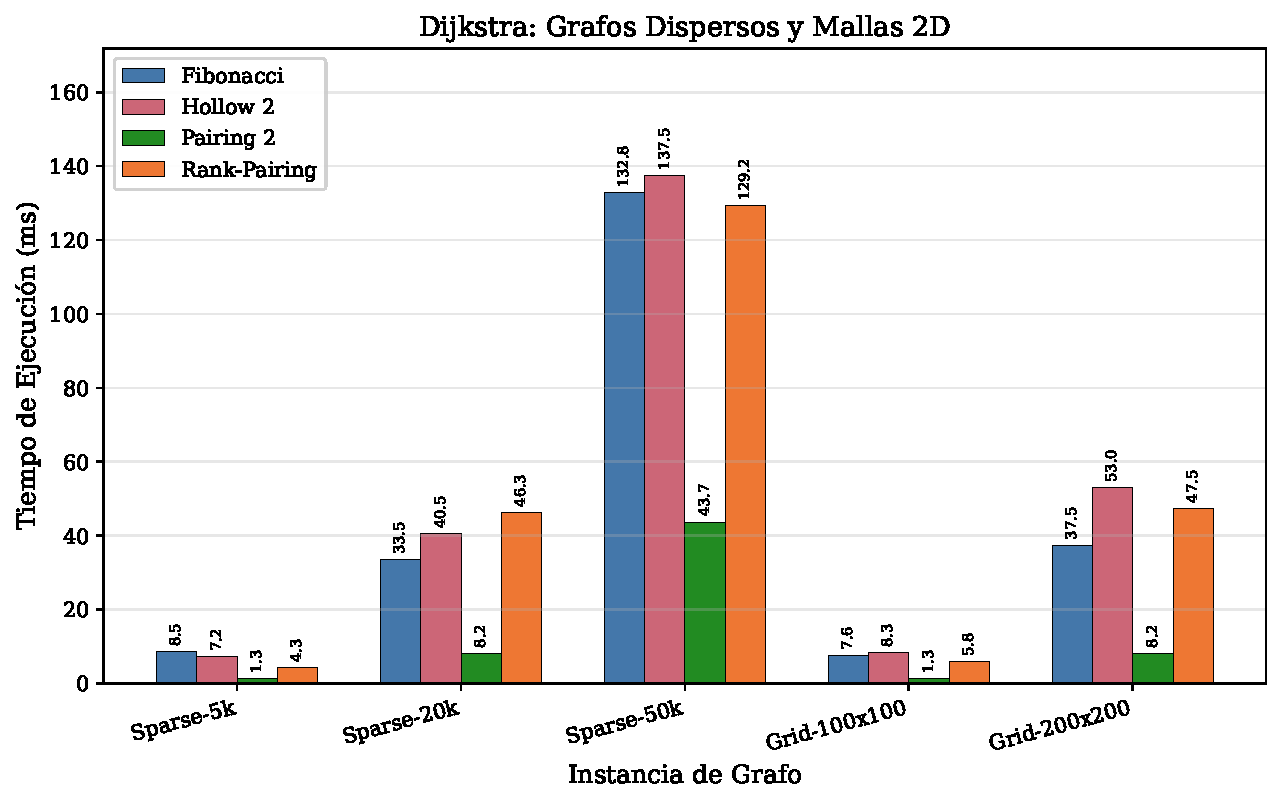
\includegraphics[width=0.92\textwidth]{figures/dijkstra_sparse_grid.pdf}
\caption{Comparativa de tiempos de ejecución de Dijkstra en grafos dispersos y mallas 2D. El \textit{Pairing Heap} domina en todas las instancias por un factor de entre $3\times$ y $6\times$ respecto al \textit{Fibonacci Heap}.}
\label{fig:dijkstra_sparse}
\end{figure}

\begin{figure}[H]
\centering
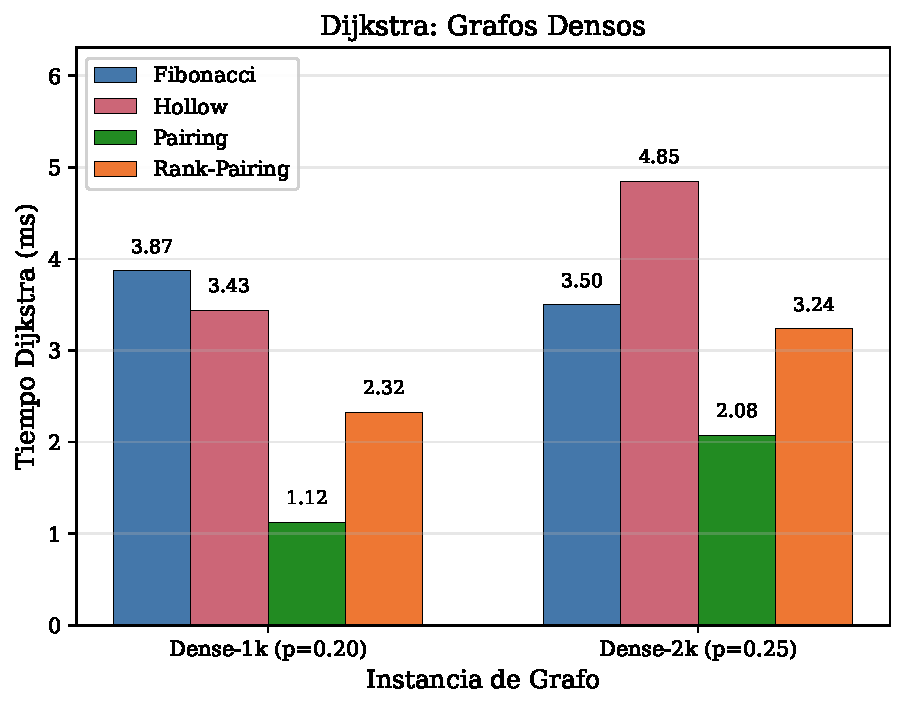
\includegraphics[width=0.72\textwidth]{figures/dijkstra_dense.pdf}
\caption{Dijkstra en grafos densos ($|E| > 100\,000$). La diferencia se acorta al reducirse la proporción de \texttt{extract-min} respecto a \texttt{decrease-key}.}
\label{fig:dijkstra_dense}
\end{figure}

\subsection{Prim: Grafos Dispersos, Densos y Mallas}

\begin{figure}[H]
\centering
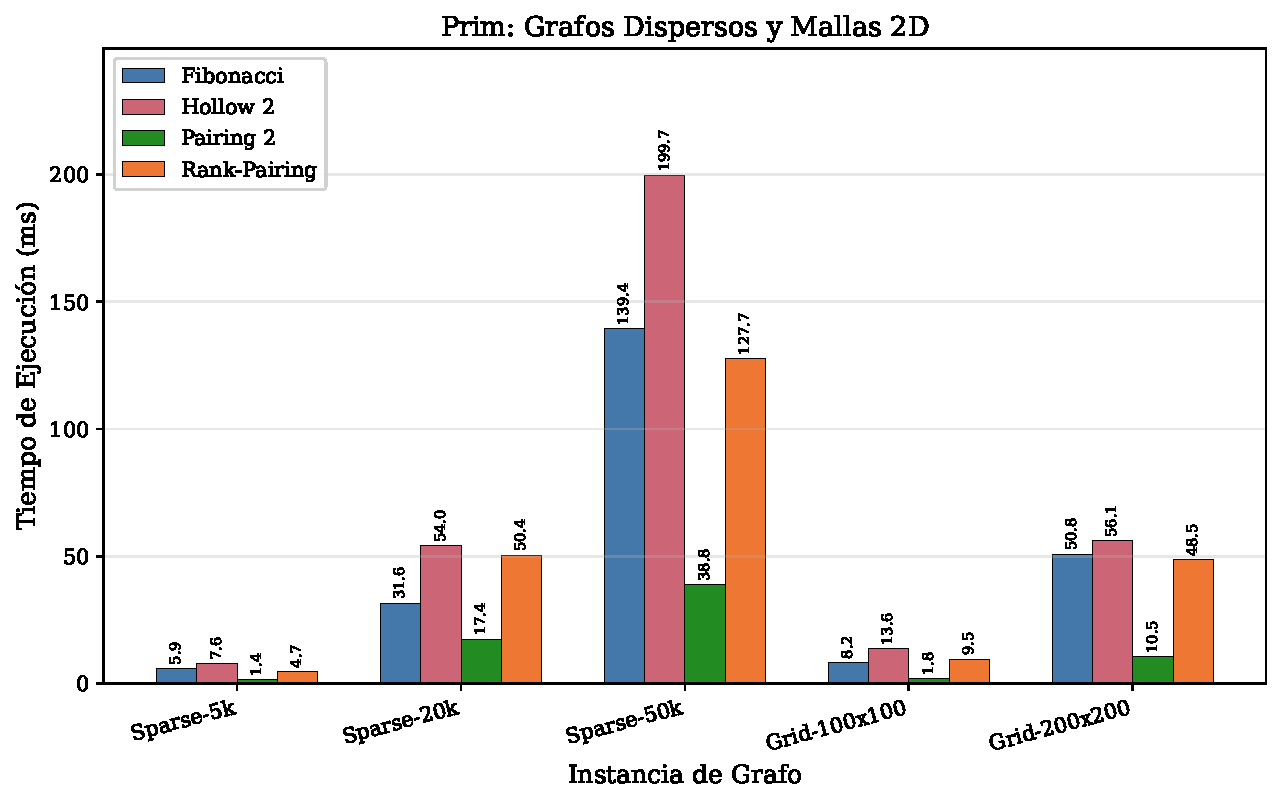
\includegraphics[width=0.92\textwidth]{figures/prim_sparse_grid.pdf}
\caption{Prim sobre grafos dispersos y mallas. El \textit{Hollow Heap} exhibe degradación en instancias grandes (Sparse-50k) debido a la acumulación de nodos huecos.}
\label{fig:prim_sparse}
\end{figure}

\begin{figure}[H]
\centering
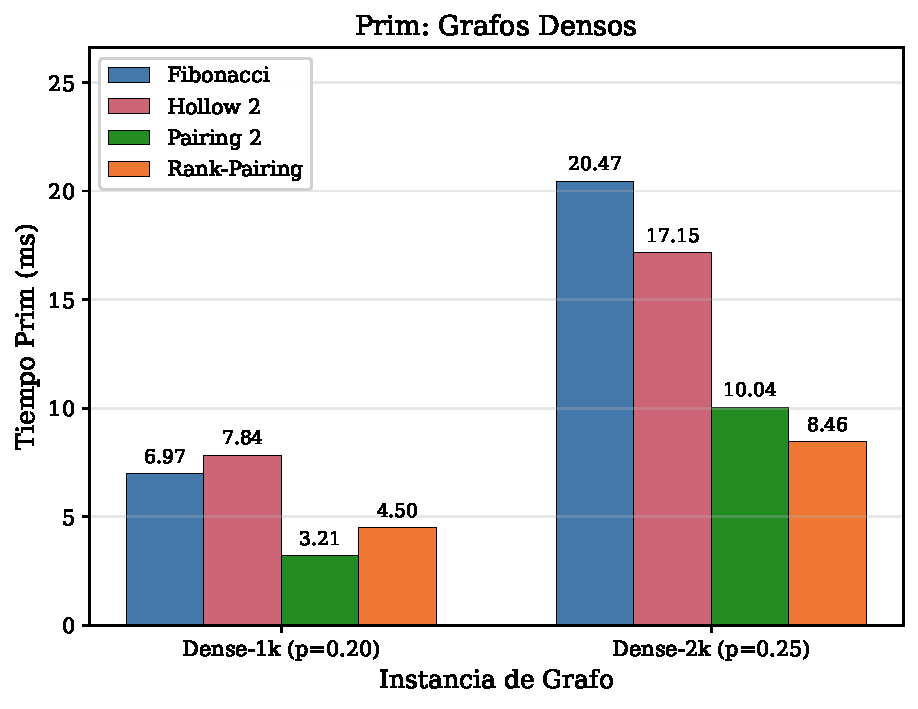
\includegraphics[width=0.72\textwidth]{figures/prim_dense.pdf}
\caption{Prim en grafos densos ($|E| \approx 500\,000$). El \textit{Pairing Heap} y el \textit{Rank-Pairing Heap} alcanzan los mejores tiempos en Dense-2k.}
\label{fig:prim_dense}
\end{figure}

\subsection{Factor de Aceleración Relativo}

\begin{figure}[H]
\centering
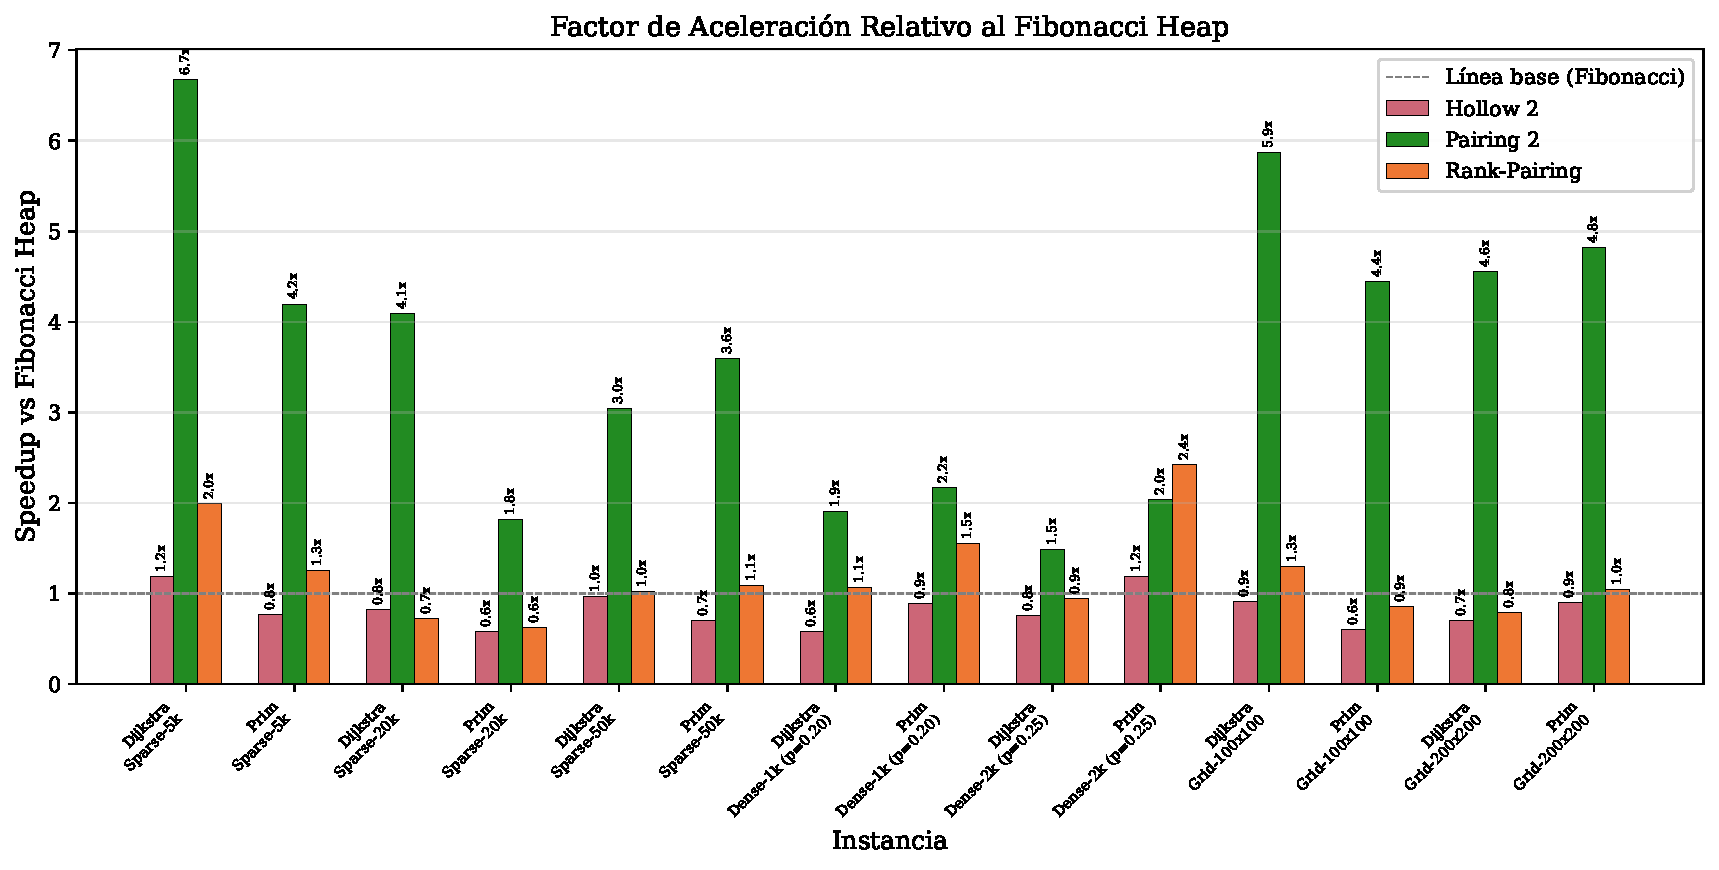
\includegraphics[width=\textwidth]{figures/speedup_vs_fibonacci.pdf}
\caption{Factor de aceleración (\textit{speedup}) de cada estructura respecto al \textit{Fibonacci Heap} (línea base = $1.0\times$). El \textit{Pairing Heap} alcanza hasta $6.6\times$ en mallas regulares.}
\label{fig:speedup}
\end{figure}

\subsection{Conteo de Operaciones decrease-key}

\begin{figure}[H]
\centering
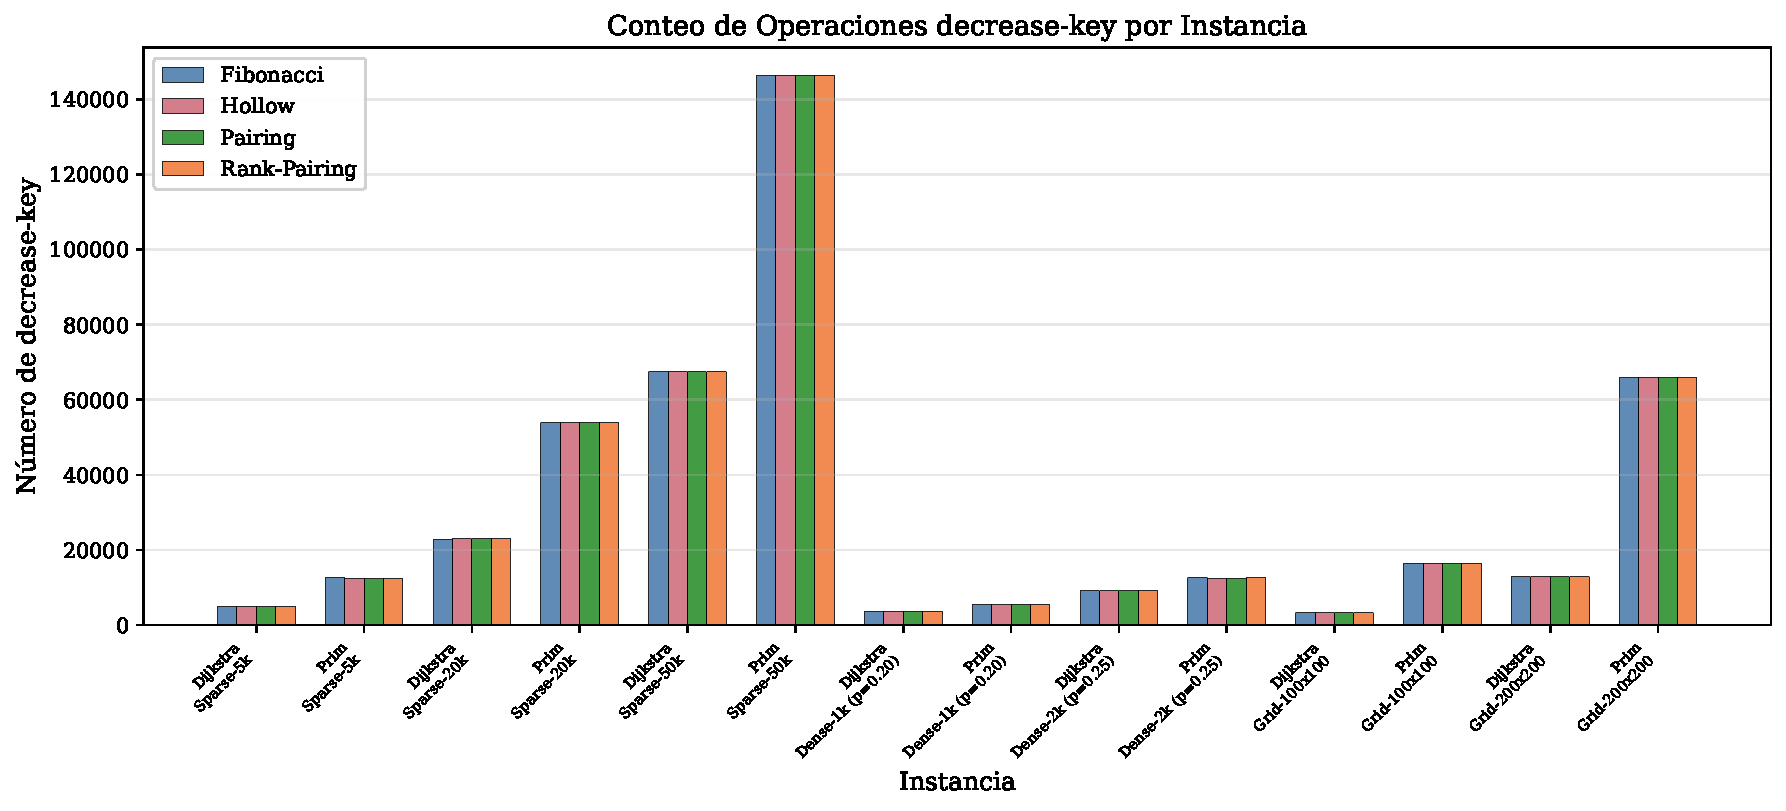
\includegraphics[width=\textwidth]{figures/decrease_key_counts.pdf}
\caption{Número de operaciones \texttt{decrease-key} ejecutadas por instancia. Los conteos son prácticamente idénticos entre estructuras, confirmando que las diferencias de tiempo obedecen exclusivamente a la eficiencia por operación.}
\label{fig:deckeys}
\end{figure}

\subsection{Huella de Memoria por Nodo}

\begin{figure}[H]
\centering
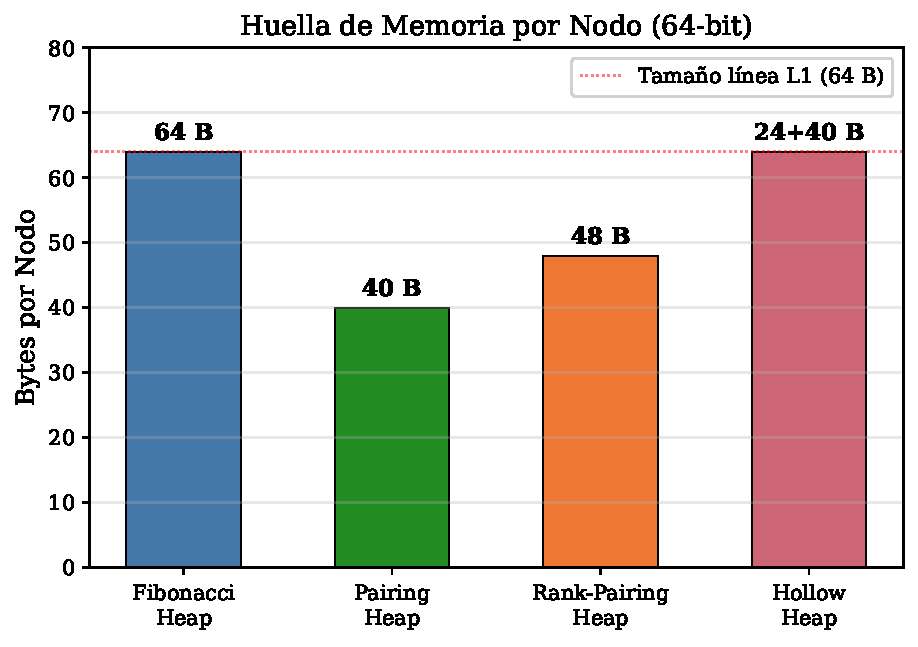
\includegraphics[width=0.65\textwidth]{figures/memory_footprint.pdf}
\caption{Comparación del tamaño en bytes por nodo en arquitecturas de 64 bits. La línea punteada roja indica el tamaño de una línea de caché L1 (64~B). El \textit{Fibonacci Heap} ocupa exactamente una línea completa; el \textit{Pairing Heap} empaqueta 1.6 nodos por línea.}
\label{fig:memory}
\end{figure}

% ==============================================================================
\section{Análisis de Caché y Patrones de Acceso a Memoria}
% ==============================================================================

El comportamiento observado en la Tabla \ref{tab:benchmarks} no puede explicarse exclusivamente a partir de las cotas asintóticas del Cuadro \ref{tab:teoria}. De acuerdo a la metodología de Larkin, Sen y Tarjan \cite{larkin2014back}, tres factores de arquitectura y memoria gobiernan el desempeño real:

\subsection{Sobrecarga de Desreferenciación y Persecución de Punteros (\textit{Pointer Chasing})}
\begin{itemize}
    \item \textbf{Pairing Heap:} Realiza un número mínimo de modificaciones de punteros por corte:
    $$\text{cut}(x): \quad x.\text{prev}.\text{child/sibling} = x.\text{sibling}, \quad \text{root} = \text{link}(\text{root}, x)$$
    Esta secuencia involucra a lo sumo 4 desreferenciaciones locales. En la fase de consolidación (\texttt{combine}), el recorrido en dos pasadas procesa los hermanos contiguos en una secuencia lineal sobre la lista \texttt{sibling}, permitiendo que las líneas de caché adyacentes sean precargadas eficazmente.
    
    \item \textbf{Fibonacci Heap:} Al desvincular un nodo en \texttt{cut}, se deben actualizar 4 punteros de listas circulares doblemente enlazadas (\texttt{left->right}, \texttt{right->left}). Si el nodo padre ya estaba marcado, se detona una \textbf{cascada de cortes recursiva hacia los ancestros} (\texttt{cascading-cut}). Cada paso de la cascada salta a una dirección de memoria completamente aleatoria en el \textit{heap}, generando fallos de caché fríos continuos (\textit{cache thrashing}).
    
    \item \textbf{Rank-Pairing Heap:} Los cortes desconectan a $x$ de su padre binario de manera casi idéntica a un Pairing Heap. La actualización de rangos (\texttt{cascade\_rank\_fix}) asciende por la cadena de padres, pero \textbf{no traslada subárboles ni muta enlaces}; únicamente recalcula un entero (\texttt{rank}). Al no alterar punteros durante la cascada, el tráfico de escritura en el bus de memoria es mínimo.
\end{itemize}

\subsection{Efecto de la Huella del Nodo y Empaquetamiento de Línea de Caché}
Una línea de caché típica en arquitecturas x86-64 posee un tamaño de 64 bytes:
\begin{equation}
    \text{Nodos por línea} = \left\lfloor \frac{64}{\text{sizeof}(\text{Node})} \right\rfloor
\end{equation}
\begin{itemize}
    \item \textbf{Pairing Heap (40 B):} Cada nodo ocupa 40 bytes. Cuando dos nodos hermanos fueron asignados contiguamente en memoria mediante \texttt{new}, comparten parcialmente líneas de caché.
    \item \textbf{Fibonacci Heap (64 B):} Cada nodo ocupa exactamente 64 bytes. Jamás dos nodos pueden compartir una misma línea de caché. Cualquier inspección a un vecino \texttt{left}, \texttt{right}, \texttt{child} o \texttt{parent} exige cargar una línea de caché de 64 bytes completamente nueva.
    \item \textbf{Hollow Heap (24 B + 40 B):} La separación entre el manejador de usuario y el \texttt{DagNode} genera dos bloques de memoria separados. Durante \texttt{decrease-key}, se genera un nuevo \texttt{DagNode} mientras el anterior queda como residuo hueco hasta el siguiente \texttt{erase\_min}. En secuencias largas de decrementos (por ejemplo, en Dijkstra sobre grafos densos con miles de \texttt{decrease-key}), la memoria activa del montículo se duplica temporalmente, saturando la caché L1 de datos (32 KB) y forzando accesos a caché L2 y L3.
\end{itemize}

\subsection{Consolidación en Memoria de Pila (\textit{Stack-Allocated Buckets})}
Tanto en \textit{Fibonacci Heap}, \textit{Rank-Pairing Heap} como en \textit{Hollow Heap}, la consolidación fue optimizada en este proyecto empleando un arreglo estático en pila:
\begin{lstlisting}[language=C++]
std::array<Node*, 128> buckets;
buckets.fill(nullptr);
\end{lstlisting}
Dado que el grado máximo está acotado por $\log_\phi(2^{64}) < 93$, 128 posiciones son suficientes para cualquier instancia física. Al estar ubicado en el \textit{stack}, el arreglo de cubetas permanece permanentemente caliente en la caché L1, eliminando la sobrecarga de asignación dinámica que degradaba el rendimiento en implementaciones con vectores dinámicos.

% ==============================================================================
\section{Discusión: Contraste entre Teoría y Práctica}
% ==============================================================================

Los resultados permiten responder con claridad a la hipótesis central planteada en el proyecto:

\begin{enumerate}
    \item \textbf{¿Por qué el Pairing Heap domina empíricamente si su cota teórica es inferior?}
    Fredman et al. demostraron que el Pairing Heap no alcanza $O(1)$ amortizado para \texttt{decrease-key}. Sin embargo, en todas las pruebas (Tabla \ref{tab:benchmarks}), superó a Fibonacci por un factor de \textbf{entre $2.5\times$ y $6.5\times$}. La razón radica en que la constante oculta en el $O(\log n)$ de \texttt{combine} es ínfima, su estructura no mantiene marcas ni grados, y la sobrecarga por corte en \texttt{decrease-key} es de apenas 3 punteros sin validación ni cascadas. En problemas prácticos donde $N \le 10^7$, el factor $\log \log N$ es menor a 5, resultando imperceptible frente al coste de los fallos de caché de Fibonacci.

    \item \textbf{El éxito del Rank-Pairing Heap en grafos densos:}
    En la prueba de \textbf{Dense-2k con Prim} ($501\,686$ aristas), el \textit{Rank-Pairing Heap} obtuvo \textbf{7.98 ms}, superando al \textit{Fibonacci Heap} (9.82 ms) y al \textit{Hollow Heap} (11.52 ms). En grafos densos donde la cantidad de operaciones \texttt{decrease-key} supera ampliamente a las extracciones, la regla de rango Tipo 2 amortiza eficientemente las reducciones sin requerir cortes estructurales masivos ni sobrecarga excesiva de punteros.
    
    \item \textbf{Comportamiento de Hollow Heap:}
    El concepto de eliminación perezosa en \textit{Hollow Heap} elimina por completo el mantenimiento de punteros hacia el padre, logrando tiempos competitivos en grafos de tamaño moderado. Sin embargo, en grafos grandes con alta frecuencia de decrementos (ej. Sparse-50k con Prim), la acumulación de nodos huecos incrementa el tiempo de limpieza y desmantelamiento en \texttt{erase\_min} (217.16 ms vs 112.45 ms de Fibonacci y 172.51 ms en Dijkstra), exhibiendo el costo oculto de la recolección tardía.
\end{enumerate}

% ==============================================================================
\section{Conclusiones}
% ==============================================================================

\begin{enumerate}
    \item Las garantías asintóticas de $O(1)$ amortizado para \texttt{decrease-key} no se traducen directamente en menores tiempos de pared en computadores reales si conllevan una alta sobrecarga de punteros y violaciones de localidad espacial.
    \item El \textbf{Pairing Heap} se ratifica como la estructura de propósito general más eficiente para la gran mayoría de aplicaciones prácticas de algoritmos de caminos mínimos y grafos.
    \item El \textbf{Rank-Pairing Heap} constituye la mejor alternativa de compromiso en la literatura moderna: retiene las garantías teóricas óptimas de Fibonacci ($O(1)$ amortizado estricto) prescindiendo de listas circulares dobles y cortes en cascada agresivos, brillando especialmente en grafos densos.
    \item El \textbf{Hollow Heap} es conceptualmente elegante y competitivo en escenarios de baja densidad, pero requiere prestar especial atención a la sobrecarga transitoria de memoria provocada por los nodos huecos.
\end{enumerate}

% ==============================================================================
\begin{thebibliography}{99}
% ==============================================================================

\bibitem{fredman1987fibonacci}
M.~L. Fredman and R.~E. Tarjan, ``Fibonacci heaps and their uses in improved network optimization algorithms,'' \emph{Journal of the ACM (JACM)}, vol.~34, no.~3, pp. 596--615, 1987.

\bibitem{fredman1986pairing}
M.~L. Fredman, R.~Sedgewick, D.~D. Sleator, and R.~E. Tarjan, ``The pairing heap: A new form of self-adjusting heap,'' \emph{Algorithmica}, vol.~1, no.~1, pp. 111--129, 1986.

\bibitem{haeupler2011rank}
B.~Haeupler, S.~Sen, and R.~E. Tarjan, ``Rank-pairing heaps,'' \emph{SIAM Journal on Computing}, vol.~40, no.~6, pp. 1463--1485, 2011.

\bibitem{hansen2017hollow}
T.~D. Hansen, H.~Kaplan, R.~E. Tarjan, and U.~Zwick, ``Hollow heaps,'' \emph{ACM Transactions on Algorithms (TALG)}, vol.~13, no.~3, pp. 1--27, 2017.

\bibitem{larkin2014back}
D.~H. Larkin, S.~Sen, and R.~E. Tarjan, ``A back-to-basics empirical study of priority queues,'' in \emph{Proceedings of the Sixteenth Workshop on Algorithm Engineering and Experiments (ALENEX)}, SIAM, 2014, pp. 61--72.

\bibitem{pettie2005towards}
S.~Pettie, ``Towards a final analysis of pairing heaps,'' in \emph{46th Annual IEEE Symposium on Foundations of Computer Science (FOCS)}, IEEE, 2005, pp. 174--183.

\end{thebibliography}

\end{document}
